% Bloque LaTeX listo para incorporar al draft en español.
% Paquetes requeridos en el preámbulo:
% \usepackage{amsmath,amssymb,booktabs,graphicx}

\subsection{Ejemplo ilustrativo}
\label{sec:i00c-illustrative-example}

Para ilustrar el efecto conjunto de las restricciones estructurales, sociales
y de balance de perfiles, se considera la instancia sintética
\texttt{I00C\_DRAFT\_ILUSTRATIVO\_27}. La instancia representa la transición
desde tres cursos de origen, $O=\{8A,8B,8C\}$, hacia tres cursos de destino,
$C=\{1M\text{-}A,1M\text{-}B,1M\text{-}C\}$, y contiene 27 estudiantes,
nueve de cada curso de origen. Todos los datos son sintéticos y el ejemplo
tiene un propósito exclusivamente metodológico; por lo tanto, sus resultados
no deben interpretarse como evidencia acerca de estudiantes o establecimientos
educacionales reales.

Cada curso de destino tiene capacidad $U_c=9$. Se fija $\alpha_o=2$ para todo
$o\in O$ y $\Delta_g=2$ para ambos grupos de género. La instancia contiene 49
nominaciones dirigidas de preferencias y ocho pares no ordenados de separación.
Las preferencias se mantienen como una componente blanda de la función objetivo:
la variable $z_i$ no se fija en uno. Se conserva, sin modificaciones, la función
objetivo ponderada de la formulación original,
\begin{equation}
  Z(\lambda_0,\lambda_1)
  = \lambda_0\left(|S|-\sum_{i\in S}z_i\right)+\lambda_1 T,
  \label{eq:i00c-weighted-objective}
\end{equation}
donde $|S|-\sum_i z_i$ corresponde al número de estudiantes que no son
asignados junto con alguno de sus pares preferidos, y $T$ es la máxima
dispersión entre los criterios académico, socioemocional y de convivencia
escolar.

\subsubsection{Solución base}
\label{sec:i00c-baseline-solution}

Para los pesos base, $\lambda_0=\lambda_1=1$, SCIP certificó una solución
óptima con brecha de optimalidad igual a cero. En esta solución, 26 de los 27
estudiantes son asignados junto con al menos un par preferido. Por consiguiente,
la componente social es
\[
  |S|-\sum_{i\in S}z_i=27-26=1.
\]
Las dispersiones reconstruidas directamente a partir de la asignación son
$F_{ac}=F_{se}=F_{cv}=14/3$, por lo que $T=14/3$. En consecuencia,
\begin{equation}
  Z(1,1)=1+\frac{14}{3}=\frac{17}{3}\approx 5.6667.
  \label{eq:i00c-baseline-value}
\end{equation}
La asignación fue verificada de manera independiente a partir de los archivos
de salida y satisface las restricciones de asignación única, capacidad,
separación, balance de género y representación mínima de los cursos de origen.

La Figura~\ref{fig:i00c-flows} presenta los flujos agregados de esta solución.
En el orden $(1M\text{-}A,1M\text{-}B,1M\text{-}C)$, la distribución por curso
de origen es
\[
  8A:(3,3,3), \qquad 8B:(4,2,3), \qquad 8C:(2,4,3).
\]
De este modo, cada curso de destino recibe nueve estudiantes y cada par
origen--destino satisface el requerimiento mínimo $\alpha_o=2$.

\begin{figure}[htbp]
  \centering
  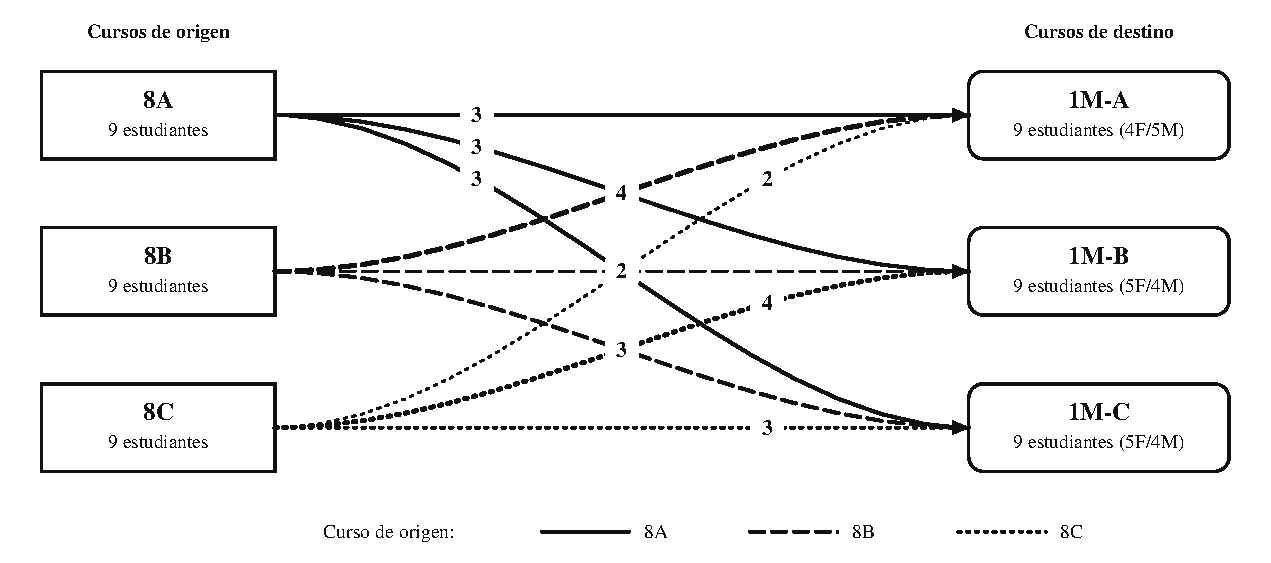
\includegraphics[width=\textwidth]{figuras/fig_i00c_flujos_origen_destino.pdf}
  \caption{Reasignación de los 27 estudiantes en la solución base del ejemplo
  ilustrativo. El tipo de línea identifica el curso de origen, el grosor es
  proporcional al número de estudiantes trasladados y el valor de cada flujo
  se indica directamente sobre el arco correspondiente. La codificación es
  monocromática y no depende del color.}
  \label{fig:i00c-flows}
\end{figure}

\subsubsection{Sensibilidad respecto de los pesos de la función objetivo}
\label{sec:i00c-lambda-sensitivity}

Para examinar el compromiso inducido por la
Ecuación~\eqref{eq:i00c-weighted-objective}, se resolvió exactamente la misma
instancia, sin modificar sus datos ni restricciones, para los siete pares de
pesos positivos
\begin{equation}
\begin{split}
\mathcal{W}=\{&(0.10,1.00),(0.25,1.00),(0.50,1.00),(1.00,1.00),\\
              &(1.00,0.50),(1.00,0.25),(1.00,0.10)\}.
\end{split}
\label{eq:i00c-weight-set}
\end{equation}
Estos pares cubren razones $\lambda_0/\lambda_1$ entre 0.1 y 10 e incluyen
la parametrización $(1,1)$ utilizada en el ejemplo. Se emplean pesos
estrictamente positivos para evitar soluciones degeneradas producidas por la
eliminación de alguna componente de la función objetivo. El ejercicio conserva
la formulación vigente de suma ponderada: no utiliza el método de
$\varepsilon$-restricción, prioridades lexicográficas ni una nueva formulación
biobjetivo.

Cada escenario fue resuelto con SCIP 10.0.2 mediante PySCIPOpt 6.2.1, utilizando
un hilo, una brecha objetivo igual a cero y un límite individual de 120 segundos.
Las siete ejecuciones finalizaron con estado óptimo y brecha final igual a cero.
Como las etiquetas de los tres cursos de destino son simétricas en esta
instancia, en los escenarios distintos al caso base se aplicó una permutación
uniforme de dichas etiquetas después de resolver, únicamente para facilitar la
comparación de los flujos. En el escenario $(1,1)$ se conservó la solución de
referencia del draft después de verificar de forma independiente que es
factible y que alcanza el mismo valor óptimo certificado por SCIP. El archivo
JSON conserva también la solución bruta seleccionada por el solver. Estas
reglas son exclusivamente de presentación: no agregan una segunda función
objetivo ni modifican el MILP.

\begingroup
\renewcommand{\tablename}{Tabla}
\begin{table}[htbp]
\centering
\caption{Sensibilidad del ejemplo ilustrativo respecto de los pesos de la función objetivo.}
\label{tab:i00c-sensibilidad-lambda}
\small
\resizebox{\textwidth}{!}{%
\begin{tabular}{lrrrrrrrrl}
\toprule
Escenario & $\lambda_0$ & $\lambda_1$ & $\lambda_0/\lambda_1$ & Satisfechos & $U$ & $T$ & $(F_{ac},F_{se},F_{cv})$ & $Z$ & Flujos 8A; 8B; 8C \\
\midrule
Balance 10:1 & 0,10 & 1,00 & 0,10 & 24/27 & 3 & 2,6667 & (2,6667; 2,6667; 2,6667) & 2,9667 & 4/2/3; 2/3/4; 3/4/2 \\
Balance 4:1 & 0,25 & 1,00 & 0,25 & 24/27 & 3 & 2,6667 & (2,6667; 2,6667; 2,6667) & 3,4167 & 4/2/3; 2/3/4; 3/4/2 \\
Balance 2:1 & 0,50 & 1,00 & 0,50 & 24/27 & 3 & 2,6667 & (2,6667; 2,6667; 2,6667) & 4,1667 & 3/4/2; 4/3/2; 2/2/5 \\
Base del draft & 1,00 & 1,00 & 1,00 & 26/27 & 1 & 4,6667 & (4,6667; 4,6667; 4,6667) & 5,6667 & 3/3/3; 4/2/3; 2/4/3 \\
Preferencias 2:1 & 1,00 & 0,50 & 2,00 & 27/27 & 0 & 6,6667 & (6,6667; 6,6667; 2,6667) & 3,3333 & 3/3/3; 3/4/2; 3/2/4 \\
Preferencias 4:1 & 1,00 & 0,25 & 4,00 & 27/27 & 0 & 6,6667 & (6,6667; 6,6667; 2,6667) & 1,6667 & 3/3/3; 3/4/2; 3/2/4 \\
Preferencias 10:1 & 1,00 & 0,10 & 10,00 & 27/27 & 0 & 6,6667 & (6,6667; 6,6667; 2,6667) & 0,6667 & 3/3/3; 3/4/2; 3/2/4 \\
\bottomrule
\end{tabular}%
}
\vspace{2pt}
\begin{minipage}{\textwidth}
\footnotesize\textit{Nota:} $U=|S|-\sum_i z_i$ es el número de estudiantes sin una preferencia satisfecha. Las dispersiones se presentan como $(F_{ac};F_{se};F_{cv})$ y los flujos, en el orden 1M-A/1M-B/1M-C.
\end{minipage}
\end{table}
\endgroup


La Tabla~\ref{tab:i00c-sensibilidad-lambda} permite distinguir tres regímenes
entre los pesos evaluados. Cuando el balance de perfiles recibe un mayor peso
relativo, con $\lambda_0/\lambda_1\leq0.5$, el modelo alcanza
$T=8/3\approx2.6667$, valor que coincide con la cota inferior aritmética para
esta instancia. El costo de este balance más estricto es una menor satisfacción
de preferencias: 24 de los 27 estudiantes tienen al menos una preferencia
satisfecha ($88.9\%$), por lo que $U=3$.

Para el par base $(1,1)$, la solución utilizada en el ejemplo ilustrativo tiene
$U=1$, una satisfacción de preferencias de $26/27$ estudiantes ($96.3\%$) y
$T=14/3$. Cuando la satisfacción de preferencias recibe un mayor peso relativo,
para las razones evaluadas $\lambda_0/\lambda_1\geq2$, los 27 estudiantes tienen
una preferencia satisfecha ($U=0$), mientras que $T$ aumenta a
$20/3\approx6.6667$. Por lo tanto, en esta instancia sintética, satisfacer la
preferencia del último estudiante requiere aceptar una mayor dispersión máxima
de perfiles.

Los resultados también muestran la existencia de soluciones óptimas múltiples.
Para $\lambda_0/\lambda_1=1$, los pares de componentes
$(U,T)=(3,8/3)$ y $(U,T)=(1,14/3)$ producen el mismo valor $Z=17/3$. En
consecuencia, la solución de la
Sección~\ref{sec:i00c-baseline-solution} es una solución óptima representativa,
pero no es única en términos de sus dos componentes objetivo. De forma análoga,
para $(\lambda_0,\lambda_1)=(1,0.5)$, los pares $(1,14/3)$ y $(0,20/3)$
producen $Z=10/3$. Asimismo, los escenarios de balance muestran que un mismo
par $(U,T)$ puede corresponder a asignaciones diferentes. Esto es coherente con
la simetría y con la existencia de óptimos múltiples en el modelo.

Este análisis de sensibilidad caracteriza la instancia ilustrativa y no debe
interpretarse como una calibración empírica de $\lambda_0$ y $\lambda_1$. La
selección de pesos para una aplicación real requeriría criterios normativos y
una validación con los actores pertinentes del proceso de decisión.
